\documentclass{standalone}
\usepackage{tikz}
\usepackage{pgfplots}
\usepackage{epstopdf} %include eps Drawings from LaTeX Drawing Programs
\usepackage{mathtools}
\newcommand{\defvar}{\vcentcolon=} %Use command /defvar for define symbol
\begin{document}
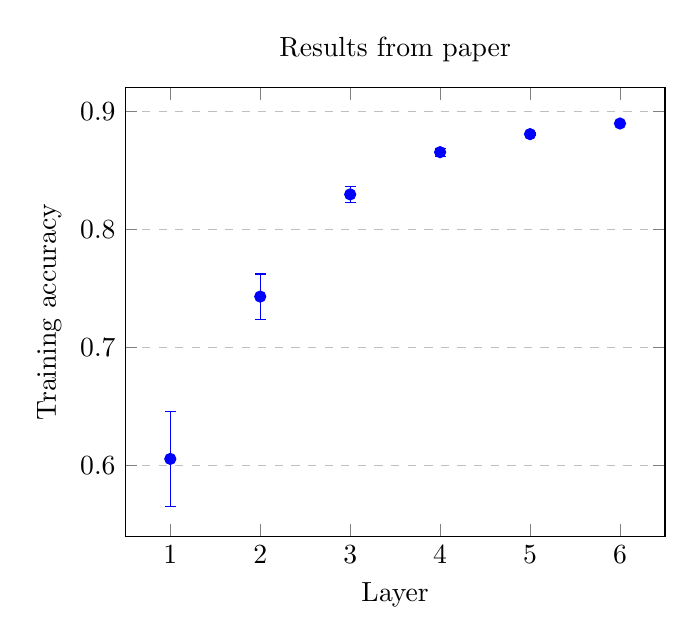
\begin{tikzpicture}
\begin{axis}[
    title={Results from paper},
    xlabel={Layer},
    ylabel={Training accuracy},
    xmin=0.5, xmax=6.5,
    ymin=0.54, ymax=0.92,
    %xtick={0,20,40,60,80,100},
    %ytick={0,20,40,60,80,100,120},
    legend style={font=\small},
    legend pos=north west,
    ymajorgrids=true,
    grid style=dashed,
]
\addplot+[
mark=*,
mark options={blue},
error bars/error bar style={blue},
only marks, error bars/.cd,
x dir=both,x explicit,
y dir=both,y explicit,
]
table[x=x,x error=xerror,y=y,y error=yerror]
{
x  xerror  y       yerror
1  0.001   0.6055  0.0403
2  0.001   0.7431  0.0191
3  0.001   0.8297  0.0068
4  0.001   0.8655  0.0033
5  0.001   0.8808  0.0015
6  0.001   0.8898  0.0000
};
%\addlegendentry[]{Druck Wasserdampf}
%\addplot [
	%restrict y to domain=0.2:3,
    %domain=-345:400, 
    %samples=300, 
    %color=red,
%]
%{-0.28516+4.99E-05*exp(-x/-36.67958)};
%\addlegendentry[]{Exponentieller Fit}
\end{axis}
\end{tikzpicture}
\end{document}

